\documentclass[12pt]{amsart}
\usepackage[left=0.5in, right=0.5in, bottom=0.75in, top=0.75in]{geometry}
\usepackage[english]{babel}
\usepackage[utf8x]{inputenc}
\usepackage{amsmath,amssymb,amsthm}
\usepackage{enumerate}
\usepackage{graphicx}

\usepackage[table,xcdraw,dvipsnames]{xcolor}
\usepackage{tikz}
\usepackage{pgfplots}
\usepgfplotslibrary{fillbetween}
\usepackage{booktabs}

\renewcommand{\thesection}{\arabic{section}}
\renewcommand{\thesubsection}{\arabic{section}.\arabic{subsection}}
\renewcommand{\thesubsubsection}{\quad(\alph{subsubsection})}

\begin{document}
\raggedbottom

\noindent{\large STAT 601 - Theory of Probability %
	- Homework 1 }
\hspace{\fill} {\large B. Hosley}
\bigskip


%%%%%%%%%%%%%%%%%%%%%%%
\setcounter{section}{1}
\setcounter{subsection}{4}
\subsection{} % 1.5
\textit{Approximately one-third of all human twins are identical (one-egg) and two-thirds are fraternal (two-egg) twins. 
	Identical twins are necessarily the same sex, with male and female being equally likely. 
	Among fraternal twins, approximately one-fourth are both female, one-fourth are both male, and half are one male and one female. 
	Finally, among all U.S. births, approximately 1 in 90 is a twin birth. Define the following events:}
	\begin{align*}
		A &= \{\text{a U.S. birth results in twin females}\} \\
		B &= \{\text{a U.S. birth results in identical twins}\} \\
		C &= \{\text{a U.S. birth results in twins}\}
	\end{align*}
	\subsubsection{} State, in words, the event \(A\cap B\cap C\). \\
	
	
	This event description corresponds to the situation in which a U.S. birth results in identical twin females.
	
	
	\subsubsection{} Find \(P(A\cap B\cap C)\). \\

	We may visualize the set interactions as follows (not to scale):

	\begin{center}
		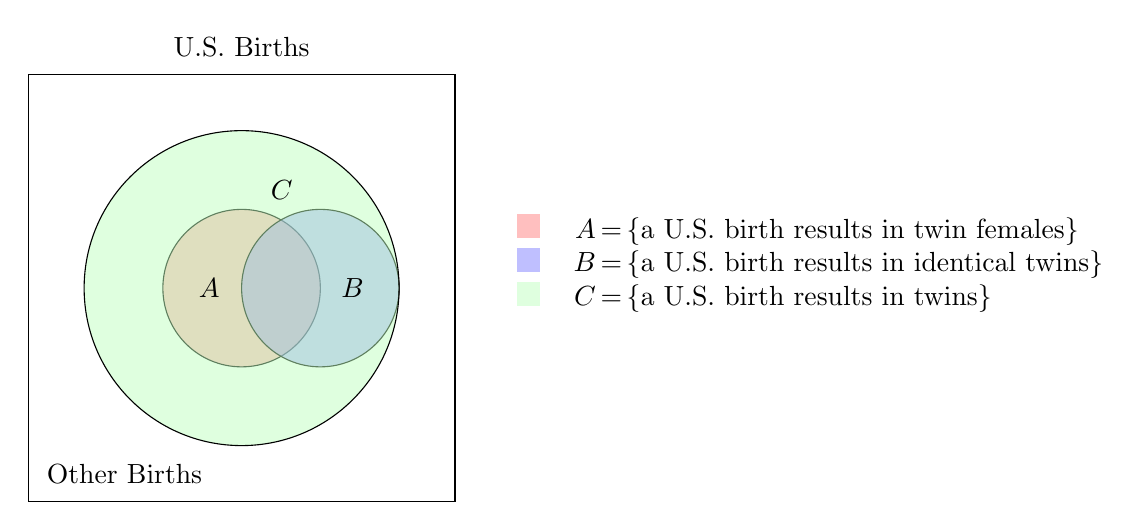
\begin{tikzpicture}
			\def\radius{1cm}
			\def\mycolorbox#1{\textcolor{#1}{\rule{2ex}{2ex}}}
			\colorlet{colorA}{red!50}
			\colorlet{colorB}{blue!50}
			\colorlet{colorC}{green!25}
			
			\coordinate (cenA);
			\coordinate[xshift=\radius] (cenB);
			\coordinate (cenC);
			
			\draw[fill=colorA,fill opacity=0.5] (cenA) circle (\radius);
			\draw[fill=colorB,fill opacity=0.5] (cenB) circle (\radius);
			\draw[fill=colorC,fill opacity=0.5] (cenC) circle (2*\radius);
			
			\draw  ([xshift=-20pt,yshift=20pt]current bounding box.north west) 
			rectangle ([xshift=20pt,yshift=-20pt]current bounding box.south east);
			
			\node[yshift=10pt] at (current bounding box.north) {U.S. Births};
			
			\node at ([xshift=4.5*\radius]current bounding box.east) 
			{
				\begin{tabular}{@{}lr@{\,=\,}l@{}}
					\mycolorbox{colorA!50} & $A$ & \{a U.S. birth results in twin females\} \\
					\mycolorbox{colorB!50} & $B$ & \{a U.S. birth results in identical twins\} \\
					\mycolorbox{colorC!50} & $C$ & \{a U.S. birth results in twins\}
				\end{tabular}
			};
			
			\node[xshift=-.4\radius] at (cenA) {$A$};
			\node[xshift=.4\radius] at (cenB) {$B$};
			\node[xshift=.5\radius,yshift=1.25*\radius] at (cenC) {$C$};
			\node[xshift=35pt,yshift=10pt] at (current bounding box.south west) {Other Births};
		\end{tikzpicture}
	\end{center}
	
We can also translate the values given in the word problem to be

$$P(C) = \frac{1}{90} ,\quad P(B|C) = \frac{1}{3} ,\quad P(A|B) = \frac{1}{2} ,\quad P(A|C\backslash B) = \frac{1}{4} ,\quad P(B^c|C) = \frac{2}{3}.$$

Then, we can calculate the intersection as

$$ P(A\cap B\cap C) \equiv P(A|B)P(B|C) P(C) = \frac{1}{540}. $$ \\[2em]

\subsection{} % 1.6
\textit{Two pennies, one with \(P\)(head) \(= u\) and one with \(P\)(head) \(= w\), are to be tossed together independently. Define}
\begin{align*}
	p_0 &= P(\text{0 heads occurs}), \\
	p_1 &= P(\text{1 heads occurs}), \\
	p_2 &= P(\text{2 heads occurs}). \\
\end{align*}
\textit{Can \(u\) and \(w\) be chosen such that \(p_0 = p_1 = p_2\)? Prove your answer.}

First, we will translate $p_n$ into the given variables,

\begin{align*}
	p_0 &= (1-u)(1-w) \\
	p_2 &= w(1-u)+u(1-w) \\
	p_3 &= uw.
\end{align*}

Then, if we assume for sake of contradiction that \(p_0 = p_1 = p_2\) we will see that

\begin{align*}
	p_0 &=  p_2\\
	(1-u)(1-w) &= uw \\
	1-u-w+uw &= uw \\
	1 &= u+w, 
\end{align*}

and thus that $w=(1-u)$. Then, using this value to substitute we can see that

\begin{align*}
	p_1 &=  p_2\\
	w(1-u)+u(1-w) &=uw \\
	(1-u)^2+u(1-(1-u)) &=u(1-u) \\
	2u(1-u) &= u(1-u) \\
	2u &= u.
\end{align*}

Thus \(p_0 = p_1 = p_2\) cannot be entirely true. \\[2em]


\setcounter{subsection}{32}
\subsection{} % 1.33
\textit{Suppose that 5\% of men and .25\% of women are color-blind. A person is chosen at random and that person is color-blind. 
	What is the probability that the person is male? (Assume males and females to be in equal numbers.)} \\

We will use Bayes' theorem where $B=$ colorblindness and $A=$ male, thus the answer to the question becomes $P(A|B)$.
Solving becomes

\begin{align*}
	P(A|B) &= \frac{P(B|A)P(A)}{P(B)} \\
	&= \frac{(0.05)(0.5)}{(0.05)(0.5)+(0.0025)(0.5)} \\
	&= \frac{(0.025)}{(0.025)+(0.00125)} \\
	&= 0.95238. \\
\end{align*} \\

\setcounter{subsection}{34}
\subsection{} % 1.35
\textit{Prove that if \(P(\cdot)\) is a legitimate probability function and \(B\) is a set with \(P (B) > 0\),
	then \(P (\cdot|B)\) also satisfies Kolmogorov’s Axioms.}

\setcounter{subsection}{36}
\subsection{} % 1.37
\textit{Here we look at some variations of Example 1.3.4}
	\subsubsection{}
	\textit{ In the warden’s calculation of Example 1.3.4 it was assumed that if \(A\) were to be
		pardoned, then with equal probability the warden would tell A that either \(B\) or \(C\)
		would die. However, this need not be the case. The warden can assign probabilities
		\(\gamma\) and \(1 − \gamma\) to these events, as shown here:} \\
	\begin{center}
		\begin{tabular}{ccc}
			\toprule
			Prisoner pardoned & Warden tells A & \\
			\midrule
			A & B dies & with probability \(\gamma\) \\
			A & C dies & with probability \(1-\gamma\) \\
			B & C dies & \\
			C & B dies & \\
			\bottomrule
		\end{tabular} \\[1.5em]
	\end{center}
	\textit{Calculate \(P(A|\mathcal W)\) as a function of \(\gamma\). For what values of \(\gamma\) is \(P(A|\mathcal W)\) less than,
		equal to, or greater than \(\frac 1 3\)?} \\
		
	Maintaining the convention that \(\mathcal W\) describes the event of the warden telling $A$ that $B$ will be executed,
	we can use Bayes' theorem to calculate \(P(A|\mathcal W)\). Given that we already have \(P(B)\) and \(P(\mathcal W|B)\) we only
	need calculate \(P(A|\mathcal W)\);
	
	\begin{align*}
		P(\mathcal W) = \frac{1}{3} \gamma + \frac{1}{3}
		= \frac{\gamma+1}{3}. \\
	\end{align*}
	
	With that in hand we may move to Bayes' theorem to show that
	
	\begin{align*}
		P(A|\mathcal W) = \frac{P(\mathcal W|A)P(A)}{P(\mathcal W)}
		= \frac{\gamma \left( \frac{1}{3} \right)}{\frac{\gamma+1}{3}}
		= \frac{\gamma}{\gamma+1}. \\
	\end{align*}
	
	This allows us to calculate that
	\begin{align*}
		\frac 1 3
		= P(A|\mathcal W) 
		&= \frac{\gamma}{\gamma+1} \\
		\gamma+1 &= 3\gamma \\
		1 &= 2\gamma. \\			
	\end{align*}
	
	Extending the equality we can also discover the inequality, which is
	
	\begin{align*}
		P(A|\mathcal W)  
		\begin{cases}
			\geq\frac{1}{3} ,& \gamma \leq \frac 1 2 \\
			=\frac 1 3 ,& \gamma = \frac 1 2 \\
			\geq\frac{1}{3} ,& \gamma \geq \frac 1 2 \\
		\end{cases}.
	\end{align*} \\

	
	\subsubsection{}
	\textit{Suppose again that \(\gamma = \frac 1 2\), as in the example. After the warden tells \(A\) that \(B\)
		will die, \(A\) thinks for a while and realizes that his original calculation was false.
		However, \(A\) then gets a bright idea. \(A\) asks the warden if he can swap fates with \(C\).
		The warden, thinking that no information has been passed, agrees to this. Prove
		that \(A\)’s reasoning is now correct and that his probability of survival has jumped to \(\frac 2 3\)!} \\
	
	We will once again use Bayes' theorem. First we will gather a few values discovered above.
	
	\begin{align*}
	P(\mathcal W) &= \frac{\gamma+1}{3} = \frac{\frac{1}{2}+1}{3} = \frac{1}{2} \\
	P(\mathcal W|C) &= 1 \\
	P(C) &= 1/3.	\\
	\end{align*}
	
	Then,
	
	\begin{align*}
		P(C|\mathcal W) = \frac{ P(\mathcal W|C) P(C)}{P(\mathcal W)}
		= \frac{1\cdot\frac{1}{3}}{\frac{1}{2}}
		= \frac{2}{3}.
	\end{align*} \\
	
\textit{A similar, but somewhat more complicated, problem, the “Monte Hall problem” is discussed by Selvin (1975). 
	The problem in this guise gained a fair amount of notoriety when it appeared in a Sunday magazine (vos Savant 1990) along with a correct
	answer but with questionable explanation. The ensuing debate was even reported on the front page of the Sunday New York Times (Tierney 1991). 
	A complete and some what amusing treatment is given by Morgan et al. (1991) [see also the response by vos Savant 1991]. 
	Chun (1999) pretty much exhausts the problem with a very thorough analysis.} \clearpage

\subsection{} % 1.38
\textit{Prove each of the following statements. (Assume that any conditioning event has positive probability.)}
	\subsubsection{} \textit{If \(P(B) = 1\), then \(P(A|B) = P(A)\) for any \(A\).} \\
	
		If \(P(B) = 1\) then it follows that \(P(B|A) = 1\). Knowing this we can prove the assertion via
		Bayes' theorem;
		
		\begin{align*}
			P(A|B) = \frac{P(B|A)P(A)}{P(B)} = \frac{1\cdot P(A)}{1} = P(A).
		\end{align*} \\
	
	
	\subsubsection{} \textit{If \(A \subset B\), then \(P(B|A) = 1\) and \(P(A|B) = P(A)/P(B)\).} \\
	
		Define \(A^\prime\) such that \(A\cup A^\prime = B\).
		Then we can illustrate that \(P(B|A) = P(A\cup A^\prime|A) = 1\).
	
		We can use this result to get the second claim using Bayes' theorem
		\begin{align*}
			P(A|B) 
			= \frac{P(B|A)P(A)}{P(B)}
			= \frac{P(A)}{P(B)}.
		\end{align*} \\
	
	\subsubsection{} \textit{If \(A\) and \(B\) are mutually exclusive, then}
		\[ P(A|A\cup B) = \frac{P(A)}{P(A) + P(B)}. \] \\
		
		We will leverage the additive property: 
		\[P(A\cup B) = P(A) + P(B) - P(A)\cap P(B)\]
		and note that mutual exclusivity implies that \(P(A)\cap P(B) = 0\).
		Next, we will observe that \(P(A\cup B|A)=1\) as \(A\subset A\cup B\). From this we can see that 
		
		\begin{align*}
			P(A|A\cup B) = \frac{P(A\cup B|A)P(A)}{P(A\cup B)}
			= \frac{1\cdot P(A)}{P(A) + P(B)}
			= \frac{P(A)}{P(A) + P(B)}.
		\end{align*} \\[1em]
		 
	\subsubsection{} \(P(A\cap B\cap C) = P(A|B\cap C) P(B|C) P(C)\).
	
	\begin{align*}
		P(A\cap B\cap C) 
		= P(A\cap (B\cap C)) 
		= P(A\cap | B\cap C) P(B\cap C) 
		= P(A\cap | B\cap C) P(B| C) P(C) \\
	\end{align*}

\clearpage
\subsection{} % 1.39
\textit{A pair of events \(A\) and \(B\) cannot be simultaneously mutually exclusive and independent.
	Prove that if \(P(A) > 0\) and \(P(B) > 0\), then:}
	\subsubsection{} \textit{If \(A\) and \(B\) are mutually exclusive, they cannot be independent.} \\
	
	Assuming \(A\) and \(B\) are mutually exclusive, then \(A\cap B = \emptyset\) and \(P(A\cap B)=0\).
	If \(A\) and \(B\) are independent then \(P(A\cap B) = P(A)P(B) = 0\),
	but since \(P(A) > 0\) and \(P(B) > 0\) then we can conclude \(P(A)P(B) \neq 0\), thus a contradiction. \\
	
	\subsubsection{} \textit{If \(A\) and \(B\) are independent, they cannot be mutually exclusive.} \\
	
	Since \(P(A) > 0\) and \(P(B) > 0\) then \(P(A)P(B) > 0\) which implies that \(P(A\cap B)>0\)
	and therefore \(P(A\cap B)\neq\emptyset\). \\
	

\setcounter{subsection}{46}
\subsection{} % 1.47
\textit{Prove that the following functions are cdfs.}
	% lim(-infty) = 0 and lim(infty) = 1
	% Strictly non-decreasing
	% Right Continuous
	\subsubsection{} \( \frac{1}{2}+\frac{1}{\pi} \tan^{-1}(x),\, x\in(-\infty,\infty) \)
	\subsubsection{} \( (1+e^{-x})^{-1},\, x\in(-\infty,\infty) \)
	\subsubsection{} \( e^{-e^{-x}},\, x\in(-\infty,\infty) \)
	\subsubsection{} \( 1-e^{-x},\, x\in(-\infty,\infty) \)
	\subsubsection{} \textit{the function defined in (1.5.6)}

\setcounter{subsection}{50}
\subsection{} % 1.51
\textit{An appliance store receives a shipment of 30 microwave ovens, 5 of which are (unknown
	to the manager) defective. The store manager selects 4 ovens at random, without
	replacement, and tests to see if they are defective. Let \(X =\) number of defectives
	found. Calculate the pmf and cdf of \(X\) and plot the cdf.}


\subsection{} % 1.52
\textit{Let \(X\) be a continuous random variable with pdf \(f(x)\) and cdf \(F(x)\). For a fixed number \(x_0\), define the function
	\[g(x) = \begin{cases}
		f(x)/[1 − F(x_0)] & x\geq x_0 \\
		0 & x < x_0.
	\end{cases} \]
	Prove that \(g(x)\) is a pdf. (Assume that \(F(x0) < 1\).)}


\subsection{} % 1.53
\textit{A certain river floods every year. Suppose that the low-water mark is set at \(1\) and the
	high-water mark \(Y\) has distribution function}
	\[ F_Y = P(Y\leq y) = 1-\frac{1}{y^2}, \quad 1\leq y<\infty. \]
	\subsubsection{} Verify \(F_Y(y)\) is a cdf.
	
	\subsubsection{} Find \(f_Y(y)\), the pdf of \(Y\).
	
	\subsubsection{} If the low-water mark is reset at \(0\) and we use a unit of measurement that is $\frac{1}{10}$ of
		that given previously, the high-water mark becomes \(Z = 10(Y − 1)\). Find \(F_Z(z)\).
		


\subsection{} % 1.54
\textit{For each of the following, determine the value of $c$ that makes $f(x)$ a pdf.}
	\subsubsection{}
	\( f(x) = c\sin x,\, 0<x<\pi/2 \)
	
	\subsubsection{}
	\( f(x) = ce^{-x|x|},\, -\infty<x<\infty \)
	


\subsection{} % 1.55
\textit{An electronic device has lifetime denoted by $T$. The device has value $V = 5$ if it fails
	before time $t = 3$; otherwise, it has value $V = 2T$. Find the cdf of $V$, if $T$ has pdf}
	\[ f_T(t) = \frac{1}{1.5}e^{-t/(1.5)},\quad t>0.\]


\end{document}